\documentclass[12pt,letterpaper]{article}
\usepackage[utf8]{inputenc}
\usepackage{tikz}
\usetikzlibrary{trees}
\usepackage[spanish, es-nodecimaldot]{babel}
\usepackage{amsmath}
\usepackage{color}
\usepackage{algorithm}
\usepackage[noend]{algpseudocode}
\renewcommand{\algorithmicrequire}{\textbf{Entrada:}}
\renewcommand{\algorithmicensure}{\textbf{Salida:}}
\usepackage{subcaption}
\usepackage{amsfonts}
\usepackage{hyperref}
 \hypersetup{
     colorlinks=true,
     linkcolor=blue,
     filecolor=blue,
     citecolor = blue,      
     urlcolor=cyan,
     }
\usepackage{amssymb}
\usepackage{listings}
\usepackage{color}

\definecolor{mygreen}{rgb}{0,0.6,0}
\definecolor{mygray}{rgb}{0.5,0.5,0.5}
\definecolor{mymauve}{rgb}{0.58,0,0.82}

\lstset{ 
  backgroundcolor=\color{white},   % choose the background color; you must add \usepackage{color} or \usepackage{xcolor}; should come as last argument
  basicstyle=\footnotesize,        % the size of the fonts that are used for the code
  breakatwhitespace=false,         % sets if automatic breaks should only happen at whitespace
  breaklines=true,                 % sets automatic line breaking
  captionpos=b,                    % sets the caption-position to bottom
  commentstyle=\color{mygreen},    % comment style
  deletekeywords={...},            % if you want to delete keywords from the given language
  escapeinside={\%*}{*)},          % if you want to add LaTeX within your code
  extendedchars=true,              % lets you use non-ASCII characters; for 8-bits encodings only, does not work with UTF-8
  firstnumber=1,                % start line enumeration with line 1000
  frame=single,	                   % adds a frame around the code
  keepspaces=true,                 % keeps spaces in text, useful for keeping indentation of code (possibly needs columns=flexible)
  keywordstyle=\color{blue},       % keyword style
  language=Octave,                 % the language of the code
  morekeywords={*,...},            % if you want to add more keywords to the set
  numbers=none,                    % where to put the line-numbers; possible values are (none, left, right)
  numbersep=5pt,                   % how far the line-numbers are from the code
  numberstyle=\tiny\color{mygray}, % the style that is used for the line-numbers
  rulecolor=\color{black},         % if not set, the frame-color may be changed on line-breaks within not-black text (e.g. comments (green here))
  showspaces=false,                % show spaces everywhere adding particular underscores; it overrides 'showstringspaces'
  showstringspaces=false,          % underline spaces within strings only
  showtabs=false,                  % show tabs within strings adding particular underscores
  stepnumber=2,                    % the step between two line-numbers. If it's 1, each line will be numbered
  stringstyle=\color{mymauve},     % string literal style
  tabsize=2,	                   % sets default tabsize to 2 spaces
  title=\lstname                   % show the filename of files included with \lstinputlisting; also try caption instead of title
}

\usepackage{amsthm}
\newtheorem{theorem}{Teorema}

\usepackage{graphicx}
\usepackage[inner=1.5 cm, outer = 1.5 cm, top=1 cm, bottom = 1.5 cm]{geometry}
\setlength{\parskip}{3mm}
\title{\textsc{Práctica 8: Modelo de urnas}}
\author{\textsc{Fabiola Vázquez}}
\renewcommand{\lstlistingname}{Código}
\setlength{\parindent}{0cm}

\begin{document}
\maketitle

\hrule
\section{Introducción}
Se tiene una simulación sobre los fenómenos de coalescencia y fragmetación de partículas que forman cúmulos. El objetivo de esta práctica \cite{elisapractica8} es determinar el porcentaje de cúmulos que pueden ser filtrados si tienen un tamaño mayor o igual que un valor específico \texttt{c}, el cual es la media del tamaño de los cúmulos iniciales. El experimento se lleva a cabo en el software R \cite{R} en un cuaderno de Jupyter \cite{jupyter}.

\section{Experimento}
Para el experimento, se consideran los parámetros \texttt{k}, que es la cantidad de cúmulos que se tiene, \texttt{n} la cantidad de partículas y \texttt{duracion} que es la cantidad de pasos que se simula. El parámetro \texttt{k} varía su valor en $\{100, 1000, 10000\}$ y \texttt{n}, que se toma como un múltiplo de \texttt{k}, varía su valor en $\{$10\texttt{k}, 20\texttt{k}, 50\texttt{k}, 100\texttt{k}, 1000\texttt{k}$\}$ y el parámetro \texttt{duracion} varía en $\{10, 25, 50, 75, 100\}$.

Al código elaborado por Schaeffer \cite{codigoelisapractica8}, se le añade el código \ref{lst:gc1} para determinar el porcentaje de cúmulos que tienen un tamaño mayor o igual \texttt{c} y que pueden ser filtrados.

\begin{lstlisting}[label=lst:gc1,caption=Cálculo del porcentaje de cúmulos filtrados., frame = single]
for (i in 1:length(freq$num)){
	if(freq$tam[i]>=c){
		cum <- c(cum, freq$num[i])
    }
}
a<-sum(cum)/sum(freq$num)
\end{lstlisting} 

\begin{figure}
 	\centering
 	\begin{subfigure}[b]{0.7\linewidth}
 		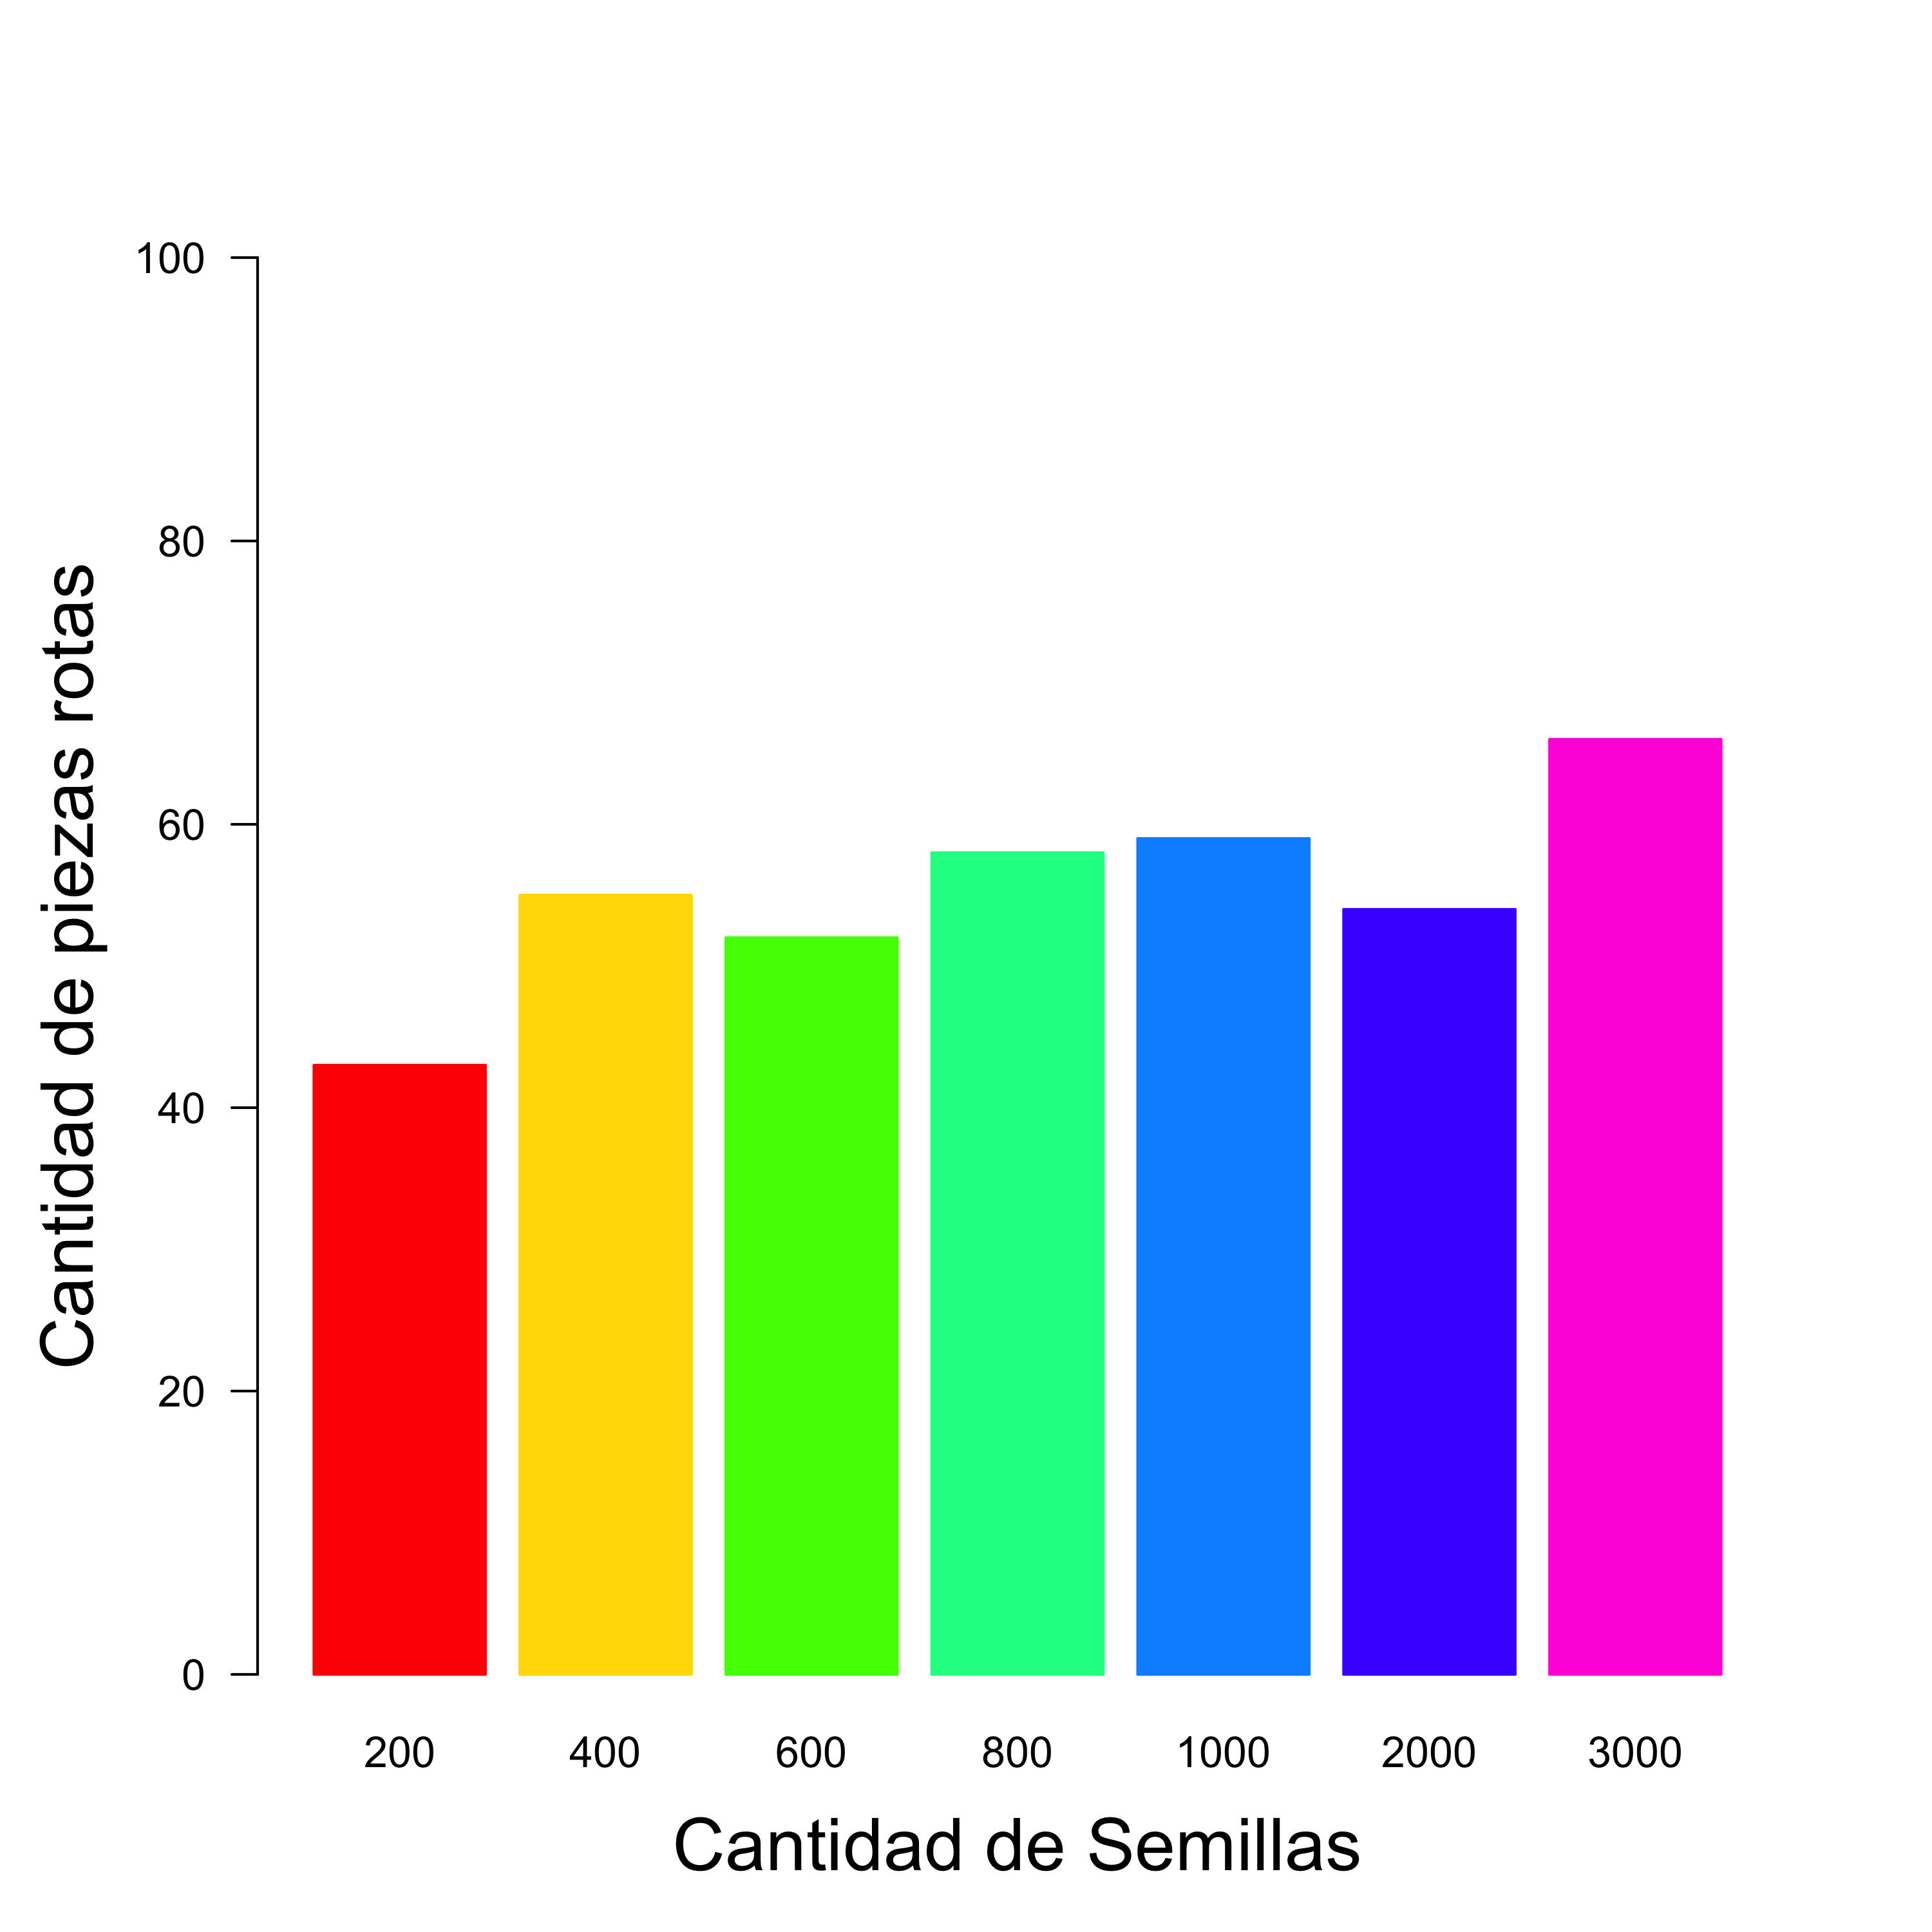
\includegraphics[width=\linewidth]{100.png}
 		 \caption{Gráficas de caja-bigote con \texttt{k} = 100.}
 		\label{100}
 	\end{subfigure}
 	\begin{subfigure}[b]{0.7\linewidth}
 		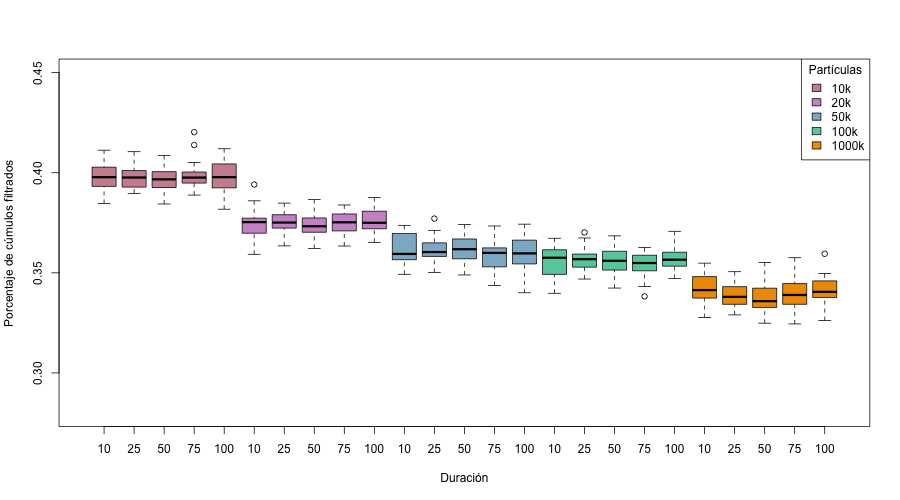
\includegraphics[width=\linewidth]{1000.png}
 		 \caption{Gráficas de caja-bigote con \texttt{k} = 1000.}
 		\label{1000}
 	\end{subfigure}
  	\begin{subfigure}[b]{0.7\linewidth}
 		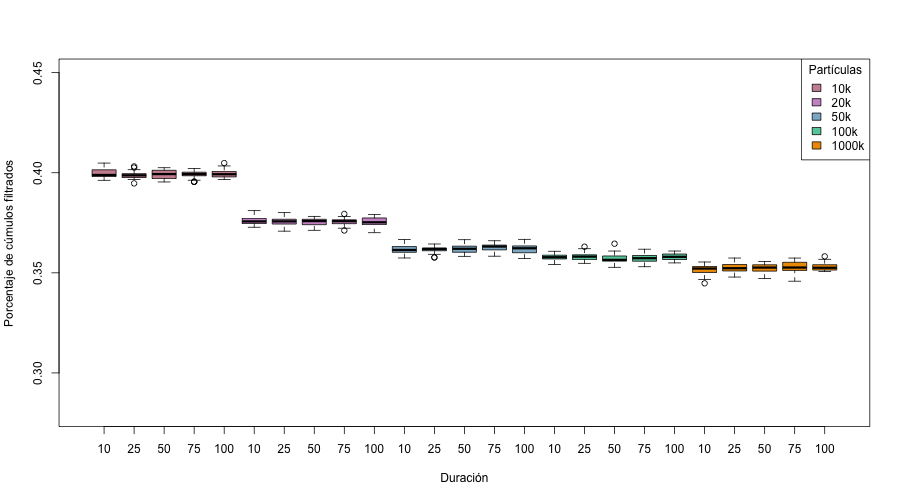
\includegraphics[width=\linewidth]{10000.png}
 		 \caption{Gráficas de caja-bigote con \texttt{k} = 10000.}
 		\label{10000}
 	\end{subfigure}
 	\caption{Gráficas de caja.}  	
\label{graficas}
 \end{figure}

En la figura \ref{graficas} se muestran las gráficas de caja-bigote de las diferentes combinaciones de los parámetros \texttt{k}, \texttt{n} y \texttt{duracion}. En la figura \ref{100} se omitió la combinación de \texttt{k}=100 cúmulos con \texttt{n}=1000\texttt{k} partículas, ya que el porcentaje de cúmulos filtrados en dicha combinación es de cero para los cinco valores de \texttt{duracion}. Como se aprecia en la figura \ref{graficas} para los diferentes valores de \texttt{k}, la diferencia es que las cajas se hacen más pequeñas pero oscilan entre los mismos valores.

\subsection{Pruebas de correlación}
Para comprobar si alguno de los parámetros influye en la cantidad de cúmulos filtrados se realizan pruebas de correlación. El cuadro \ref{corr} muestra los valores $p$ obtenidos en las pruebas, de los cuales solo el del parámetro \texttt{k} es menor que 0.05, es decir que existe correlación entre la cantidad de cúmulos y el porcentaje de cúmulos filtrados, pero dado que el coeficiente de correlación es 0.2310 la correlación que existe es débil. Los parámetros \texttt{n} y \texttt{duracion} no afectan al porcentaje de cúmulos filtrados.
\begin{table}
\centering
\caption{Resultados de las pruebas de correlación.}
\label{corr}
\begin{tabular}{rrr}
  \hline
 Parámetro & valor $p$ & Coeficiente de correlación\\ 
  \hline
Cúmulos \texttt{k}& $2.2\times 10^{-16}$ &   0.2310 \\ 
Partículas \texttt{n}&  0.1809 &   0.0309 \\ 
\texttt{duracion}& 0.9211 & -0.0022 \\ 
\hline
\end{tabular}
\end{table}

\section{Reto 1}
En el reto 1 se pide determinar en cuál iteración el porcentaje de cúmulos filtrados alcanza un punto máximo, para esto se modifica la función añadiendo el código \ref{lst:gc2}.

\begin{lstlisting}[label=lst:gc2,caption=Iteración en la cuál el porcentaje de cúmulos filtrados es máximo., frame = single]
cum <- c()
	for (i in 1:length(freq$num)){
		if(freq$tam[i]>=c){
			cum <- c(cum, freq$num[i])
		}
	}
	a<-sum(cum)/sum(freq$num)
	porcentajes[paso] <- a
}
return(which.max(porcentajes))
\end{lstlisting} 
Se realiza el experimento variando el valor de \texttt{k} en $\{100, 1000, 100000\}$ y \texttt{n} en $\{$10\texttt{k}, 100\texttt{k}, 1000\texttt{k}$\}$ y se fija el parámetro \texttt{duracion} en 50.
\begin{figure}
 	\centering
 	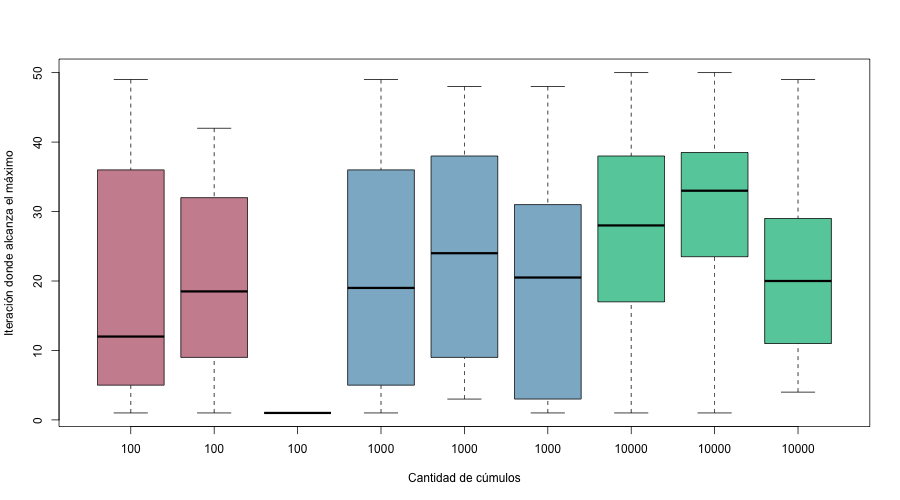
\includegraphics[width=\linewidth]{reto1.png}
 		 \caption{Gráficas de caja-bigote.}
 		\label{reto}
\end{figure}
 	
\bibliographystyle{plain} 
\bibliography{Referencias}


\end{document} 